\documentclass{standalone}
\usepackage{tikz}
\usetikzlibrary{patterns, positioning}

\begin{document}
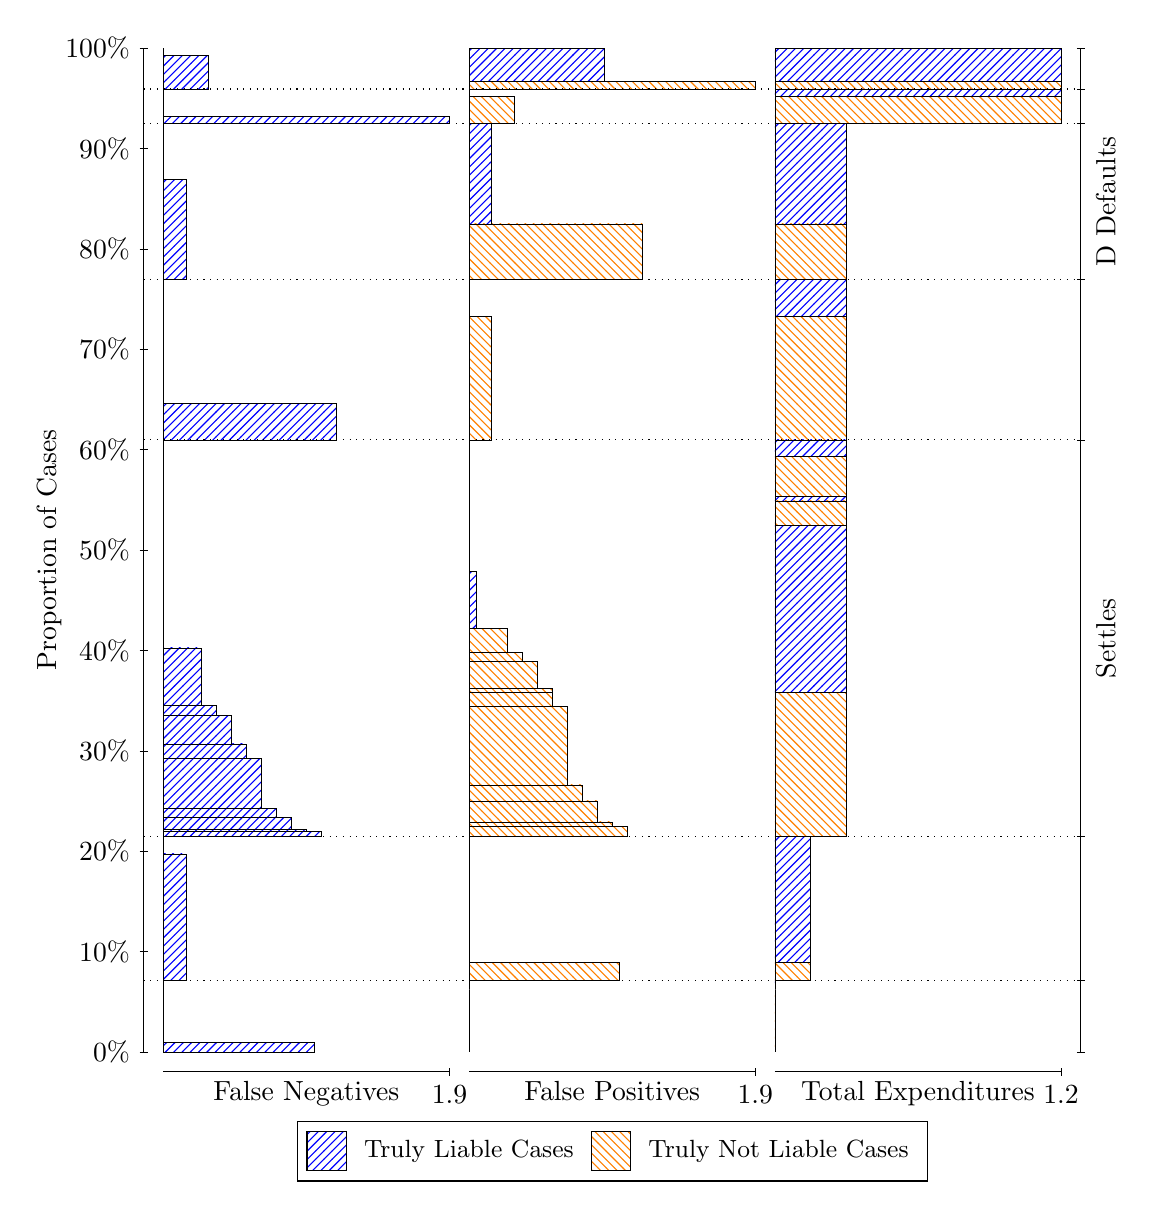
\begin{tikzpicture}
\draw[black, very thin] (1.5,1.75) -- (1.5,14.5);
\node[rotate=90, anchor=center] at (0.3, 8.125) {Proportion of Cases};
\draw[black, very thin] (1.45,1.75) -- (1.55,1.75);
\node[anchor=east] at (1.45, 1.75) {0\%};
\draw[black, very thin] (1.45,3.025) -- (1.55,3.025);
\node[anchor=east] at (1.45, 3.025) {10\%};
\draw[black, very thin] (1.45,4.3) -- (1.55,4.3);
\node[anchor=east] at (1.45, 4.3) {20\%};
\draw[black, very thin] (1.45,5.575) -- (1.55,5.575);
\node[anchor=east] at (1.45, 5.575) {30\%};
\draw[black, very thin] (1.45,6.85) -- (1.55,6.85);
\node[anchor=east] at (1.45, 6.85) {40\%};
\draw[black, very thin] (1.45,8.125) -- (1.55,8.125);
\node[anchor=east] at (1.45, 8.125) {50\%};
\draw[black, very thin] (1.45,9.4) -- (1.55,9.4);
\node[anchor=east] at (1.45, 9.4) {60\%};
\draw[black, very thin] (1.45,10.675) -- (1.55,10.675);
\node[anchor=east] at (1.45, 10.675) {70\%};
\draw[black, very thin] (1.45,11.95) -- (1.55,11.95);
\node[anchor=east] at (1.45, 11.95) {80\%};
\draw[black, very thin] (1.45,13.225) -- (1.55,13.225);
\node[anchor=east] at (1.45, 13.225) {90\%};
\draw[black, very thin] (1.45,14.5) -- (1.55,14.5);
\node[anchor=east] at (1.45, 14.5) {100\%};

\draw[black, very thin] (13.4,1.75) -- (13.4,14.5);
\draw[black, very thin] (13.35,1.75) -- (13.45,1.75);
\node[anchor=west] at (13.35, 1.75) {};
\draw[black, very thin] (13.35,2.6617) -- (13.45,2.6617);
\node[anchor=west] at (13.35, 2.6617) {};
\draw[black, very thin] (13.35,4.4861) -- (13.45,4.4861);
\node[anchor=west] at (13.35, 4.4861) {};
\draw[black, very thin] (13.35,9.5238) -- (13.45,9.5238);
\node[anchor=west] at (13.35, 9.5238) {};
\draw[black, very thin] (13.35,11.562) -- (13.45,11.562);
\node[anchor=west] at (13.35, 11.562) {};
\draw[black, very thin] (13.35,13.539) -- (13.45,13.539);
\node[anchor=west] at (13.35, 13.539) {};
\draw[black, very thin] (13.35,13.98) -- (13.45,13.98);
\node[anchor=west] at (13.35, 13.98) {};
\draw[black, very thin] (13.35,14.5) -- (13.45,14.5);
\node[anchor=west] at (13.35, 14.5) {};

\draw[black, very thin, pattern color=blue, pattern=north east lines] (1.75,1.75) rectangle (3.6623,1.8693);
\draw[black, very thin, pattern color=orange, pattern=north west lines] (1.75,1.8693) rectangle (1.75,2.6617);
\draw[black, very thin, pattern color=blue, pattern=north east lines] (1.75,2.6617) rectangle (2.0368,4.2648);
\draw[black, very thin, pattern color=orange, pattern=north west lines] (1.75,4.2648) rectangle (1.75,4.4861);
\draw[black, very thin, pattern color=blue, pattern=north east lines] (1.75,4.4861) rectangle (3.7579,4.5467);
\draw[black, very thin, pattern color=blue, pattern=north east lines] (1.75,4.5467) rectangle (3.5667,4.579);
\draw[black, very thin, pattern color=blue, pattern=north east lines] (1.75,4.579) rectangle (3.3754,4.7278);
\draw[black, very thin, pattern color=blue, pattern=north east lines] (1.75,4.7278) rectangle (3.1842,4.8475);
\draw[black, very thin, pattern color=blue, pattern=north east lines] (1.75,4.8475) rectangle (2.993,5.4809);
\draw[black, very thin, pattern color=blue, pattern=north east lines] (1.75,5.4809) rectangle (2.8018,5.662);
\draw[black, very thin, pattern color=blue, pattern=north east lines] (1.75,5.662) rectangle (2.6105,6.0211);
\draw[black, very thin, pattern color=blue, pattern=north east lines] (1.75,6.0211) rectangle (2.4193,6.1538);
\draw[black, very thin, pattern color=blue, pattern=north east lines] (1.75,6.1538) rectangle (2.2281,6.8807);
\draw[black, very thin, pattern color=orange, pattern=north west lines] (1.75,6.8807) rectangle (1.75,9.5238);
\draw[black, very thin, pattern color=blue, pattern=north east lines] (1.75,9.5238) rectangle (3.9491,9.991);
\draw[black, very thin, pattern color=orange, pattern=north west lines] (1.75,9.991) rectangle (1.75,11.562);
\draw[black, very thin, pattern color=blue, pattern=north east lines] (1.75,11.562) rectangle (2.0368,12.834);
\draw[black, very thin, pattern color=orange, pattern=north west lines] (1.75,12.834) rectangle (1.75,13.539);
\draw[black, very thin, pattern color=blue, pattern=north east lines] (1.75,13.539) rectangle (5.3833,13.634);
\draw[black, very thin, pattern color=orange, pattern=north west lines] (1.75,13.634) rectangle (1.75,13.98);
\draw[black, very thin, pattern color=blue, pattern=north east lines] (1.75,13.98) rectangle (2.3237,14.405);
\draw[black, very thin, pattern color=orange, pattern=north west lines] (1.75,14.405) rectangle (1.75,14.5);
\draw[black, very thin, pattern color=orange, pattern=north west lines] (5.6333,1.75) rectangle (5.6333,2.5424);
\draw[black, very thin, pattern color=blue, pattern=north east lines] (5.6333,2.5424) rectangle (5.6333,2.6617);
\draw[black, very thin, pattern color=orange, pattern=north west lines] (5.6333,2.6617) rectangle (7.5456,2.883);
\draw[black, very thin, pattern color=blue, pattern=north east lines] (5.6333,2.883) rectangle (5.6333,4.4861);
\draw[black, very thin, pattern color=orange, pattern=north west lines] (5.6333,4.4861) rectangle (7.6412,4.6147);
\draw[black, very thin, pattern color=orange, pattern=north west lines] (5.6333,4.6147) rectangle (7.45,4.6724);
\draw[black, very thin, pattern color=orange, pattern=north west lines] (5.6333,4.6724) rectangle (7.2588,4.9393);
\draw[black, very thin, pattern color=orange, pattern=north west lines] (5.6333,4.9393) rectangle (7.0675,5.141);
\draw[black, very thin, pattern color=orange, pattern=north west lines] (5.6333,5.141) rectangle (6.8763,6.1342);
\draw[black, very thin, pattern color=orange, pattern=north west lines] (5.6333,6.1342) rectangle (6.6851,6.3173);
\draw[black, very thin, pattern color=orange, pattern=north west lines] (5.6333,6.3173) rectangle (6.6851,6.3633);
\draw[black, very thin, pattern color=orange, pattern=north west lines] (5.6333,6.3633) rectangle (6.4939,6.7093);
\draw[black, very thin, pattern color=orange, pattern=north west lines] (5.6333,6.7093) rectangle (6.3026,6.8218);
\draw[black, very thin, pattern color=orange, pattern=north west lines] (5.6333,6.8218) rectangle (6.1114,7.1292);
\draw[black, very thin, pattern color=blue, pattern=north east lines] (5.6333,7.1292) rectangle (5.7289,7.8561);
\draw[black, very thin, pattern color=blue, pattern=north east lines] (5.6333,7.8561) rectangle (5.6333,9.5238);
\draw[black, very thin, pattern color=orange, pattern=north west lines] (5.6333,9.5238) rectangle (5.9202,11.095);
\draw[black, very thin, pattern color=blue, pattern=north east lines] (5.6333,11.095) rectangle (5.6333,11.562);
\draw[black, very thin, pattern color=orange, pattern=north west lines] (5.6333,11.562) rectangle (7.8325,12.268);
\draw[black, very thin, pattern color=blue, pattern=north east lines] (5.6333,12.268) rectangle (5.9202,13.539);
\draw[black, very thin, pattern color=orange, pattern=north west lines] (5.6333,13.539) rectangle (6.207,13.886);
\draw[black, very thin, pattern color=blue, pattern=north east lines] (5.6333,13.886) rectangle (5.6333,13.98);
\draw[black, very thin, pattern color=orange, pattern=north west lines] (5.6333,13.98) rectangle (9.2667,14.075);
\draw[black, very thin, pattern color=blue, pattern=north east lines] (5.6333,14.075) rectangle (7.3544,14.5);
\draw[black, very thin, pattern color=orange, pattern=north west lines] (9.5167,1.75) rectangle (9.5167,2.5424);
\draw[black, very thin, pattern color=blue, pattern=north east lines] (9.5167,2.5424) rectangle (9.5167,2.6617);
\draw[black, very thin, pattern color=orange, pattern=north west lines] (9.5167,2.6617) rectangle (9.9708,2.883);
\draw[black, very thin, pattern color=blue, pattern=north east lines] (9.5167,2.883) rectangle (9.9708,4.4861);
\draw[black, very thin, pattern color=orange, pattern=north west lines] (9.5167,4.4861) rectangle (10.425,6.3173);
\draw[black, very thin, pattern color=blue, pattern=north east lines] (9.5167,6.3173) rectangle (10.425,8.4419);
\draw[black, very thin, pattern color=orange, pattern=north west lines] (9.5167,8.4419) rectangle (10.425,8.7493);
\draw[black, very thin, pattern color=blue, pattern=north east lines] (9.5167,8.7493) rectangle (10.425,8.8099);
\draw[black, very thin, pattern color=orange, pattern=north west lines] (9.5167,8.8099) rectangle (10.425,9.3144);
\draw[black, very thin, pattern color=blue, pattern=north east lines] (9.5167,9.3144) rectangle (10.425,9.5238);
\draw[black, very thin, pattern color=orange, pattern=north west lines] (9.5167,9.5238) rectangle (10.425,11.095);
\draw[black, very thin, pattern color=blue, pattern=north east lines] (9.5167,11.095) rectangle (10.425,11.562);
\draw[black, very thin, pattern color=orange, pattern=north west lines] (9.5167,11.562) rectangle (10.425,12.268);
\draw[black, very thin, pattern color=blue, pattern=north east lines] (9.5167,12.268) rectangle (10.425,13.539);
\draw[black, very thin, pattern color=orange, pattern=north west lines] (9.5167,13.539) rectangle (13.15,13.886);
\draw[black, very thin, pattern color=blue, pattern=north east lines] (9.5167,13.886) rectangle (13.15,13.98);
\draw[black, very thin, pattern color=orange, pattern=north west lines] (9.5167,13.98) rectangle (13.15,14.075);
\draw[black, very thin, pattern color=blue, pattern=north east lines] (9.5167,14.075) rectangle (13.15,14.5);
\draw[black, dotted] (1.5,2.6617) -- (13.4,2.6617);
\draw[black, dotted] (1.5,4.4861) -- (13.4,4.4861);
\draw[black, dotted] (1.5,9.5238) -- (13.4,9.5238);
\draw[black, dotted] (1.5,11.562) -- (13.4,11.562);
\draw[black, dotted] (1.5,13.539) -- (13.4,13.539);
\draw[black, dotted] (1.5,13.98) -- (13.4,13.98);
\draw[black, very thin] (1.75,1.5) -- (5.3833,1.5);
\node[anchor=north] at (3.5667, 1.5) {False Negatives};
\draw[black, very thin] (5.3833,1.45) -- (5.3833,1.55);
\node[anchor=north] at (5.3833, 1.45) {1.9};

\draw[black, very thin] (5.6333,1.5) -- (9.2667,1.5);
\node[anchor=north] at (7.45, 1.5) {False Positives};
\draw[black, very thin] (9.2667,1.45) -- (9.2667,1.55);
\node[anchor=north] at (9.2667, 1.45) {1.9};

\draw[black, very thin] (9.5167,1.5) -- (13.15,1.5);
\node[anchor=north] at (11.333, 1.5) {Total Expenditures};
\draw[black, very thin] (13.15,1.45) -- (13.15,1.55);
\node[anchor=north] at (13.15, 1.45) {1.2};



\node[black, centered, rotate=90] at (13.72, 7.0049) {Settles};

\node[black, centered, rotate=90] at (13.72, 12.551) {D Defaults};



\draw (7.449999999999999,1.5) node[draw=none] (baseCoordinate) {};
\begin{scope}[align=center]
        \matrix[scale=0.5, draw=black, below=0.5cm of baseCoordinate, nodes={draw}, column sep=0.1cm]{
            \node[rectangle, draw, minimum width=0.5cm, minimum height=0.5cm, pattern=north east lines, pattern color=blue] {}; &
            \node[draw=none, font=\small] (B) {Truly Liable Cases}; &
            \node[rectangle, draw, minimum width=0.5cm, minimum height=0.5cm, pattern=north west lines, pattern color=orange] {}; &
            \node[draw=none, font=\small] (B) {Truly Not Liable Cases}; \\
            };
\end{scope}

\end{tikzpicture}
\end{document}